\documentclass[a4paper,12pt,twoside]{memoir}

% Castellano
\usepackage[spanish,es-tabla]{babel}
\selectlanguage{spanish}
\usepackage[utf8]{inputenc}
\usepackage[T1]{fontenc}
\usepackage{lmodern} % Scalable font
\usepackage{microtype}
\usepackage{placeins}

\RequirePackage{booktabs}
\RequirePackage[table]{xcolor}
\RequirePackage{xtab}
\RequirePackage{multirow}

% Links
\usepackage[colorlinks]{hyperref}
\hypersetup{
	allcolors = {red}
}

% Ecuaciones
\usepackage{amsmath}

% Rutas de fichero / paquete
\newcommand{\ruta}[1]{{\sffamily #1}}

% Párrafos
\nonzeroparskip


% Imagenes
\usepackage{graphicx}
\newcommand{\imagen}[2]{
	\begin{figure}[!h]
		\centering
		\includegraphics[width=0.9\textwidth]{#1}
		\caption{#2}\label{fig:#1}
	\end{figure}
	\FloatBarrier
}

\newcommand{\imagenflotante}[2]{
	\begin{figure}%[!h]
		\centering
		\includegraphics[width=0.9\textwidth]{#1}
		\caption{#2}\label{fig:#1}
	\end{figure}
}



% El comando \figura nos permite insertar figuras comodamente, y utilizando
% siempre el mismo formato. Los parametros son:
% 1 -> Porcentaje del ancho de página que ocupará la figura (de 0 a 1)
% 2 --> Fichero de la imagen
% 3 --> Texto a pie de imagen
% 4 --> Etiqueta (label) para referencias
% 5 --> Opciones que queramos pasarle al \includegraphics
% 6 --> Opciones de posicionamiento a pasarle a \begin{figure}
\newcommand{\figuraConPosicion}[6]{%
  \setlength{\anchoFloat}{#1\textwidth}%
  \addtolength{\anchoFloat}{-4\fboxsep}%
  \setlength{\anchoFigura}{\anchoFloat}%
  \begin{figure}[#6]
    \begin{center}%
      \Ovalbox{%
        \begin{minipage}{\anchoFloat}%
          \begin{center}%
            \includegraphics[width=\anchoFigura,#5]{#2}%
            \caption{#3}%
            \label{#4}%
          \end{center}%
        \end{minipage}
      }%
    \end{center}%
  \end{figure}%
}

%
% Comando para incluir imágenes en formato apaisado (sin marco).
\newcommand{\figuraApaisadaSinMarco}[5]{%
  \begin{figure}%
    \begin{center}%
    \includegraphics[angle=90,height=#1\textheight,#5]{#2}%
    \caption{#3}%
    \label{#4}%
    \end{center}%
  \end{figure}%
}
% Para las tablas
\newcommand{\otoprule}{\midrule [\heavyrulewidth]}
%
% Nuevo comando para tablas pequeñas (menos de una página).
\newcommand{\tablaSmall}[5]{%
 \begin{table}
  \begin{center}
   \rowcolors {2}{gray!35}{}
   \begin{tabular}{#2}
    \toprule
    #4
    \otoprule
    #5
    \bottomrule
   \end{tabular}
   \caption{#1}
   \label{tabla:#3}
  \end{center}
 \end{table}
}

%
% Nuevo comando para tablas pequeñas (menos de una página).
\newcommand{\tablaSmallSinColores}[5]{%
 \begin{table}[H]
  \begin{center}
   \begin{tabular}{#2}
    \toprule
    #4
    \otoprule
    #5
    \bottomrule
   \end{tabular}
   \caption{#1}
   \label{tabla:#3}
  \end{center}
 \end{table}
}

\newcommand{\tablaApaisadaSmall}[5]{%
\begin{landscape}
  \begin{table}
   \begin{center}
    \rowcolors {2}{gray!35}{}
    \begin{tabular}{#2}
     \toprule
     #4
     \otoprule
     #5
     \bottomrule
    \end{tabular}
    \caption{#1}
    \label{tabla:#3}
   \end{center}
  \end{table}
\end{landscape}
}

%
% Nuevo comando para tablas grandes con cabecera y filas alternas coloreadas en gris.
\newcommand{\tabla}[6]{%
  \begin{center}
    \tablefirsthead{
      \toprule
      #5
      \otoprule
    }
    \tablehead{
      \multicolumn{#3}{l}{\small\sl continúa desde la página anterior}\\
      \toprule
      #5
      \otoprule
    }
    \tabletail{
      \hline
      \multicolumn{#3}{r}{\small\sl continúa en la página siguiente}\\
    }
    \tablelasttail{
      \hline
    }
    \bottomcaption{#1}
    \rowcolors {2}{gray!35}{}
    \begin{xtabular}{#2}
      #6
      \bottomrule
    \end{xtabular}
    \label{tabla:#4}
  \end{center}
}

%
% Nuevo comando para tablas grandes con cabecera.
\newcommand{\tablaSinColores}[6]{%
  \begin{center}
    \tablefirsthead{
      \toprule
      #5
      \otoprule
    }
    \tablehead{
      \multicolumn{#3}{l}{\small\sl continúa desde la página anterior}\\
      \toprule
      #5
      \otoprule
    }
    \tabletail{
      \hline
      \multicolumn{#3}{r}{\small\sl continúa en la página siguiente}\\
    }
    \tablelasttail{
      \hline
    }
    \bottomcaption{#1}
    \begin{xtabular}{#2}
      #6
      \bottomrule
    \end{xtabular}
    \label{tabla:#4}
  \end{center}
}

%
% Nuevo comando para tablas grandes sin cabecera.
\newcommand{\tablaSinCabecera}[5]{%
  \begin{center}
    \tablefirsthead{
      \toprule
    }
    \tablehead{
      \multicolumn{#3}{l}{\small\sl continúa desde la página anterior}\\
      \hline
    }
    \tabletail{
      \hline
      \multicolumn{#3}{r}{\small\sl continúa en la página siguiente}\\
    }
    \tablelasttail{
      \hline
    }
    \bottomcaption{#1}
  \begin{xtabular}{#2}
    #5
   \bottomrule
  \end{xtabular}
  \label{tabla:#4}
  \end{center}
}



\definecolor{cgoLight}{HTML}{EEEEEE}
\definecolor{cgoExtralight}{HTML}{FFFFFF}

%
% Nuevo comando para tablas grandes sin cabecera.
\newcommand{\tablaSinCabeceraConBandas}[5]{%
  \begin{center}
    \tablefirsthead{
      \toprule
    }
    \tablehead{
      \multicolumn{#3}{l}{\small\sl continúa desde la página anterior}\\
      \hline
    }
    \tabletail{
      \hline
      \multicolumn{#3}{r}{\small\sl continúa en la página siguiente}\\
    }
    \tablelasttail{
      \hline
    }
    \bottomcaption{#1}
    \rowcolors[]{1}{cgoExtralight}{cgoLight}

  \begin{xtabular}{#2}
    #5
   \bottomrule
  \end{xtabular}
  \label{tabla:#4}
  \end{center}
}


















\graphicspath{ {./img/} }

% Capítulos
\chapterstyle{bianchi}
\newcommand{\capitulo}[2]{
	\setcounter{chapter}{#1}
	\setcounter{section}{0}
	\chapter*{#2}
	\addcontentsline{toc}{chapter}{#2}
	\markboth{#2}{#2}
}

% Apéndices
\renewcommand{\appendixname}{Apéndice}
\renewcommand*\cftappendixname{\appendixname}

\newcommand{\apendice}[1]{
	%\renewcommand{\thechapter}{A}
	\chapter{#1}
}

\renewcommand*\cftappendixname{\appendixname\ }

% Formato de portada
\makeatletter
\usepackage{xcolor}
\newcommand{\tutor}[1]{\def\@tutor{#1}}
\newcommand{\course}[1]{\def\@course{#1}}
\definecolor{cpardoBox}{HTML}{E6E6FF}
\def\maketitle{
  \null
  \thispagestyle{empty}
  % Cabecera ----------------
\noindent
\includegraphics[width=\textwidth]{cabecera}\vspace{1cm}%
  \vfill
  % Título proyecto y escudo informática ----------------
  \colorbox{cpardoBox}{%
    \begin{minipage}{.8\textwidth}
      \vspace{.5cm}\Large
      \begin{center}
      \textbf{TFG del Grado en Ingeniería Informática}\vspace{.6cm}\\
      \textbf{\LARGE\@title{}}
      \end{center}
      \vspace{.2cm}
    \end{minipage}

  }%
  \hfill\begin{minipage}{.20\textwidth}
    
\includegraphics[width=\textwidth]{escudoInfor}
  \end{minipage}
  \vfill
  % Datos de alumno, curso y tutores ------------------
  \begin{center}%
  {%
    \noindent\LARGE
    Presentado por \@author{}\\ 
    en Universidad de Burgos --- \@date{}\\
    Tutor: \@tutor{}\\
  }%
  \end{center}%
  \null
  \cleardoublepage
  }
\makeatother

\newcommand{\nombre}{Nombre del alumno} %%% cambio de comando

% Datos de portada
\title{título del TFG}
\author{\nombre}
\tutor{nombre tutor}
\date{\today}

\begin{document}

\maketitle


\newpage\null\thispagestyle{empty}\newpage


%%%%%%%%%%%%%%%%%%%%%%%%%%%%%%%%%%%%%%%%%%%%%%%%%%%%%%%%%%%%%%%%%%%%%%%%%%%%%%%%%%%%%%%%
\thispagestyle{empty}


\noindent
\includegraphics[width=\textwidth]{cabecera}\vspace{1cm}

\noindent D. nombre tutor, profesor del departamento de nombre departamento, área de nombre área.

\noindent Expone:

\noindent Que el alumno D. \nombre, con DNI dni, ha realizado el Trabajo final de Grado en Ingeniería Informática titulado título de TFG. 

\noindent Y que dicho trabajo ha sido realizado por el alumno bajo la dirección del que suscribe, en virtud de lo cual se autoriza su presentación y defensa.

\begin{center} %\large
En Burgos, {\large \today}
\end{center}

\vfill\vfill\vfill

% Author and supervisor
\begin{minipage}{0.45\textwidth}
\begin{flushleft} %\large
Vº. Bº. del Tutor:\\[2cm]
D. nombre tutor
\end{flushleft}
\end{minipage}
\hfill
\begin{minipage}{0.45\textwidth}
\begin{flushleft} %\large
Vº. Bº. del co-tutor:\\[2cm]
D. nombre co-tutor
\end{flushleft}
\end{minipage}
\hfill

\vfill

% para casos con solo un tutor comentar lo anterior
% y descomentar lo siguiente
%Vº. Bº. del Tutor:\\[2cm]
%D. nombre tutor


\newpage\null\thispagestyle{empty}\newpage




\frontmatter

% Abstract en castellano
\renewcommand*\abstractname{Resumen}
\begin{abstract}
En este primer apartado se hace una \textbf{breve} presentación del tema que se aborda en el proyecto.
\end{abstract}

\renewcommand*\abstractname{Descriptores}
\begin{abstract}
Palabras separadas por comas que identifiquen el contenido del proyecto Ej: servidor web, buscador de vuelos, android \ldots
\end{abstract}

\clearpage

% Abstract en inglés
\renewcommand*\abstractname{Abstract}
\begin{abstract}
A \textbf{brief} presentation of the topic addressed in the project.
\end{abstract}

\renewcommand*\abstractname{Keywords}
\begin{abstract}
keywords separated by commas.
\end{abstract}

\clearpage

% Indices
\tableofcontents

\clearpage

\listoffigures

\clearpage

\listoftables
\clearpage

\mainmatter
\capitulo{1}{Introducción}

La eficiencia\cite{Eficiencia} en el mundo informático, es un termino fundamental y con mucho peso, que condiciona en la gran mayoría de ocasiones todo lo relacionado a este. Cuanta mayor eficiencia menos recursos se gastan para poder realizar un objetivo y estos recursos pueden ser utilizados para otras metas. 
La búsqueda de una buena eficiencia tiene una gran importancia dentro del ámbito laboral, donde cada recurso ahorrado puede ser fundamental, para el desarrollo de otras tareas. Un gran ejemplo de esto son los sistemas de tiempo real, donde el tiempo de respuesta debe ser mínimo, lo que hace del tiempo un recurso muy valioso, por lo cual la eficiencia de este recurso es esencial\\

En este caso nos vamos a centrar especialmente en la eficiencia aplicada a código Python, ya que es un lenguaje muy utilizado, ofrece muchas posibilidades de desarrollo y la eficiencia, es algo que se puede aplicar a casi cualquier campo conocido.
Para poder medir la eficiencia de un código hecho en lenguaje Python, primero se tendrá que empezar por determinar y desarrollar que es lo que hace que un código sea mas eficiente que otro y el como conseguir esa información.\\

A la primera pregunta la respuesta sería, "depende". Ya que según la finalidad para la que haya sido creado un programa, esta determina que factores hacen que el  programa se considere mas eficiente. Por ello existen diferentes métricas\cite{TiposEficiencia} para según que casos.\\

He aquí algunas de ellas:
\begin{itemize}
	\item Medir el tiempo de ejecución: Esta es la forma de medir la eficiencia más utilizada, esto se debe a la facilidad de llevarla a cabo, pero como gran inconveniente se podría decir que es una manera la cual devuelve resultados difícilmente repetibles. Esto es por la gran influencia que tienen algunos factores externos en los resultados que puede devolver. El mayor de estos factores son las condiciones de pruebas donde se ejecuta el código del programa, ya que si hacemos una ejecución en un mismo ordenador pero en momentos diferentes, es muy probable que algoritmos con una cierta complejidad tarde mas en ser ejecutados en un momento que en el otro. Esto se debe a que con este método para poder sacar resultados con una gran fiabilidad habría que tener un gran control sobre el entorno, lo cual requiere de una gran preparación previa.
	\item Complejidad O\cite{O} Esta forma realmente nos sirve para conocer la complejidad del código, ya que mide el numero de iteraciones que hace un programa, pero por otra parte no se llega a considerar lo que tarda en ejecutar cada iteración en concreto.
	
	\item Cuenta de Operaciones: Esta métrica se basa en contar el numero de operaciones que son necesarias en la ejecución del código. No es tan fácil de llevarla a cabo como la métrica de medir el tiempo, pero a cambio los resultados son repetibles.

\end{itemize}

La métrica elegida para ser implementada en la herramienta de este trabajo a sido la cuenta de operaciones\\
 
Se a decidido implementar la medición con operaciones por ser una manera de obtener soluciones invariables sea cual sea el entorno en el que se haga y devuelve datos con una profundidad suficiente como para poder hacer todos los análisis que se requieran. \\

Otra ventaja de utilizar esta medición es que se puede obtener la complejidad O de un programa al hacer varios análisis de un mismo fichero con diferentes valores cada vez.

En el caso de este trabajo se ha decidido que para conseguir la información de cuantas operaciones hay en la ejecución de un programa se utilizara un interprete\cite{interprete}, que como bien su nombre indica, será el responsable de interpretar el código que forma el programa y tras hacerle unas modificaciones nos guardara  la información que se desea. 




\capitulo{2}{Objetivos del proyecto}

\section{Objetivos del Proyecto}

\subsection{Objetivo general}


Desarrollar un software capaz de dar la información necesaria para realizar un análisis de eficiencia sobre un código de extension .py.
\begin{itemize}
	\item Poder hacer análisis de un código python a través del calculo de operaciones.
	\item Mostrar esa información de una manera agradable y entendible.
\end{itemize}


\subsection{Objetivos funcionales}
	\begin{itemize}
	\item El usuario podrá elegir el tipo de análisis que quiera realizar: de un fichero individual o comparando varios fichero.
	\item El usuario podrá modificar la información resultante, eligiendo las operaciones que saldrán.
	\item El usuario puede cambiar la métrica de los análisis, decidiendo como pondera cada tipo de operación
	\item El usuario podrá realizar varios análisis sin necesidad de salir de la herramienta
	\item(Exportar la información?)
\end{itemize}


\subsection{Objetvios técnicos}
	\begin{itemize}
	\item Obtener el numero de operaciones a través del análisis por parte del interprete
	\item Diseñar una manera de guardas los niveles de eficiencia de cada tipo de operación.
	\item Obtener los datos finales con los que realizar la  gráficas a través de la ponderación
	\item Utilizar Tkinter para realizar la interfaz de la herramienta
	\item Utilizar Matplotlib  para generar las gráficas tras los respectivos análisis
	\item funcionamiento de ByteCode en Python
\end{itemize}

\capitulo{3}{Conceptos teóricos}


Algunos conceptos teóricos de \LaTeX \footnote{Créditos a los proyectos de Álvaro López Cantero: Configurador de Presupuestos y Roberto Izquierdo Amo: PLQuiz}.

\section{Fundamentos Básicos}

\subsection{La eficiencia}

La eficiencia vista desde un ámbito general se definiría como el uso racionado de los recursos para conseguir un objetivo x. Esta definición puede ser aplicada a cualquier ámbito en el que se hable de eficiencia pero en el caso de este proyecto se aplicara esta definición en el ámbito computacional.
La definición citada anteriormente menciona la palabra recursos, en el ámbito que estamos tratando, cuando se habla de recursos la palabra que más suele asociarse es tiempo. Esto no quiere decir que sea la única medida de eficiencia, ni mucho menos, también se podría poner como recurso el espacio en memoria, pero el tiempo suele ser el recurso que más condiciona y la gente más en cuenta tiene en las características de los  programas.\\
Aquí llegamos a la razón de existir de este proyecto, cómo medimos lo que tarda un programa en ejecutarse de manera fiable? La manera más extendida para hacer esto, es ejecutar el programa que se desee y esperar a que termine, contado el tiempo pasado desde el comienzo hasta el final de este. Esta manera a pesar de ser sencilla, a la hora de la verdad es muy poco fiable. Para que los resultados obtenidos por este método sean considerados verídicos se tendría que asegurar que el entorno de pruebas tenga unas condiciones idóneas, como por ejemplo que el procesador que del ordenador donde se ejecuta el programa no este gastando recursos en otros procesos que estén activos en segundo plano. El problema de esto es que conseguir un entorno así muchas veces no es tarea fácil. Y como respuesta a este problema surge la idea principal de este proyecto, medir la eficiencia de un programa de una manera fiable, que no se vea afectado por factores externos a este.\\
Para lograr un método métrico para la eficiencia de un programa sin que su valor se vea afectado por el cuándo y dónde se haga el análisis, se decidió hacerlo a través de las operaciones que se ejecutan en el código del programa. Tras esto una vez se obtengan estas operaciones, se hará una ponderación a cada tipo de operación según el nivel de complejidad que se les declare. 

\subsection{El interprete}

Un interprete es un programa que analiza y ejecuta el código de otro programa instrucción a instrucción. Esta es la manera con la que se pueden detectar los diferentes elementos que componen un programa. Al realizar este trabajo en Python hay que comentar antes que el interprete se trata de una maquina de pila, lo que no deja de ser una maquina virtual que emula el funcionamiento de un ordenador. El funcionamiento principal de este se basa en almacenar y gestionar información que va recogiendo en las diversas pilas que tiene, para de esta manera poder hacer sus operaciones.\\
El interprete elegido para esta practica se trata de ByteRun, un interprete hecho en código python y para código python. Este fue elegido por ser un interprete que fue creado con el objetivo principal el aprendizaje, lo cual conlleva que su complejidad no sea muy alta y por lo tanto es relativamente fácil implementar nuevas funcionalidades en este. Por otro lado en contra parte de esa baja complejidad hay que mencionar que ByteRun no es un intérprete muy rápido, como por ejemplo podría ser Cpython, pero como en este trabajo el principal requisito que se busca en un interprete es el de poder implementar nuevas funcionalidades en este para conseguir una forma de poder detectar las operaciones ejecutadas y guardarlas. El ByteRun era una opción muy acertada que se adaptaba perfectamente a los requisitos del desarrollo.


\subsection{Bytecode}.
El ByteRun al ser un interprete de Python, no analiza directamente el código de alto nivel, lo que este analiza es un código intermedio llamado Bytecode.\\ El ByteCode se trata de un código intermedio sacado a través de la traducción de un código de alto nivel al ser tratado por una serie de procesos (lexer,compiller...). Para sacar este código intermedio se ha utilizado un modulo de Python que  actúa de desensamblador y descompone el código de alto nivel. 




\section{De código a Tiempo Computacional}

Una vez explicados los conceptos anteriores se para a contar los pasos llevados a cabo para conseguir traducir el código de alto nivel a una medida con la que se pueda medir la eficiencia,  el cual en el caso de este trabajo se ha optado por los ciclos de reloj.\\
Los pasos para hacer la transformación son los siguientes:\\
\begin{enumerate}
	\item Transformar el código de alto nivel a ByteCode a través del compilador (dis).
	\item El interprete traduce y ejecuta el ByteCode.
	\item Mientras el interprete ejecuta el ByteCode, se va obteniendo el diccionario de operaciones.
	\item Hacer la ponderación de los valores recogidos en el diccionario de operaciones con los procesadores teóricos para obtener el tiempo computacional.
\end{enumerate}

\imagen{Pasos}{Flow diagram to transform the high-level code to computational time}

\subsection{1º Paso: Obtención del ByteCode}.

Como ya se ha  comentado antes el ByteCode se trata  de un código intermedio sacado  a partir de la intervención de un compilador, para conseguir esto se cuenta con un modulo de Python llamado Dis que hace esta labor de comipilador.\\
De primeras el aspecto de este código se trata de una serie de bytes que a simple vista una persona no podría entender.\\


\begin{figure}[htb]
\centering
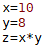
\includegraphics[width=2cm, height=3cm]{Codigo_alto_nivel}
\caption{Ejemplo de un código de alto nivel} \label{fig:horizonte}
\end{figure}

Pero el modulo Dis, cuenta con una función que permite ver el ByteCode en una especie de lenguaje ensamblador, lo cual resulta muy útil para entender la estructura del código.\\

\imagen{ByteCode}{Ejemplo del ByteCode en vista ensamblador}

La forma de entender este tipo de código es la siguiente:\\

Como ejemplo usaremos la primera fila donde se encuentra la instrucción "LOAD CONTS", la primera columna muestra el número 1 que representa la línea donde está la instrucción en el código de Python, la segunda columna es un índice que indica que la instrucción "LOAD CONTS", en En este caso, está en la posición 0, la tercera columna es el nombre de la instrucción en sí misma, mostrándola con un nombre comprensible para una persona, la cuarta columna indica la posición de ese argumento en la pila y la última columna muestra cuál es el argumento para la instrucción.\\

\subsection{2º Paso: Obtención del ByteCode}.
Una vez obtenido el Bytecode entra en , el interprete, en nuestro caso el ByteRun, es capaz de ir analizando y ejecutando el bytecode obtenido. .

\subsection{3º Paso: El Diccinario de procesos}.
El ByteRun no es capaz ir almacenando las operaciones que va traduciendo. En este momento es donde se debe implementar una nueva funcionalidad en el interprete para que sea capaz de hacer esto, para así mas tarde poder hacer un calculo de la eficiencia

Cuando el ByteRun lee una instrucción y lo primero que tiene que hacer es identificar que tipo de instrucción esta leyendo, hay muchos tipos diferentes desde un "LOAD", a un "LOOP", o un "ADD", pero a nosotros no nos interesan todas las instrucciones, solo queremos almacenar aquellas que son consideradas por nosotros como "operaciones", o lo que es lo mismo, instrucciones que necesiten de algun tipo de calculo por parte del procesador, y que por lo tanto tenga un tiempo de ejecución.\\

Por suerte para nosotros el interprete ya hace distinciones entre los diferentes tipos de instrucciones y guarda en una lista todos aquellos valores en los cuales requiere hacer una operación.\\

Aprovechando esto, cada vez que alguno de esas instrucciones es llamada guardamos el nombre que que tiene esta al ser visualizado el bytecode mediante el modulo dis en un diccionario, el cual decidimos llamar diccionario de operaciones.\\

Este diccionario tiene la siguiente estructura:\\

\begin{table}[htbp]
\begin{center}
\begin{tabular}{|l|l|}
\hline
Operación & Contador \\
\hline \hline
ADD int int & X \\ \hline
ADD int flo & X \\ \hline
MULTIPLY int int & X \\ \hline
MULTIPLY str int & X \\ \hline
DIVIDE int int & X \\ \hline
\end{tabular}
\caption{ejemplo de la estructura básica del diccionario de operaciones.}

\label{tabla:sencilla}
\end{center}
\end{table}
Se trata de un diccionario compuesto por una lista de clave primaria, y los componentes de esta lista son los siguiente:
\begin{itemize}
	\item Nombre de la operación detectada por la interfaz
	\item Primeras 3 Iniciales del tipo del primer operador 
	\item Primeras 3 Iniciales del tipo del segundo operador 
\end{itemize}




Esta estructura para las keys del diccionario se basa en el hecho de que un operación necesita de dos valores con los que operar, y dependiendo de el tipo de estos valores, dos mismas operaciones con diferentes valores, pueden llegar a tener nivel de eficiencia mucho mas bajo o alto que el otro. \\

Según el ByteRun va analizando todo el código cuando detecta una instrucción dentro de la lista de operaciones este llama a una función, que en caso de no tener ninguna entrada de esa operación y sus respectivos operadores la genera y pone de valor un 1. Posteriormente si se va encontrando mas operaciones iguales en vez de crear otra entrada en el diccionario de operaciones, incrementa en 1 el valor enlazado con la clave que la corresponde.\\

De esta manera cuando el ByteRun acaba de analizar todas las operaciones, conseguimos tener un diccionario con todas las operaciones que han surgido a lo largo de la ejecución del programa.\\

\subsection{4º Paso: Ponderación}.

Pero con solo tener los tipos de operaciones no es suficiente. Para hacer un análisis de la eficiencia es necesario saber el nivel de eficiencia que dispone cada tipo de operación, ya que no todas las operaciones tiene la misma complejidad y el procesador necesita hacer mas cálculos para ejecutarlos. Esto se consigue gracias a el procesador teórico.\\

\subsubsection{Procesadores Teóricos}
El procesador teórico tiene la función de darle un nivel de eficiencia a cada tipo de operación. Se le puso este nombre por ser la parte que simula la complejidad que le supondría a un determinado procesador, de esta manera según los valores que se guarden en el procesador se pueden simular diferentes tipos de entornos.\\

Estos procesadores se tratan de unos ficheros de tipo .csv que guardan una matriz, llamada matriz de traducción, la cual esta hecha de tal tiene una estructura pensada para poder sacar mas los  niveles de eficiencia  que guarda en cada celda según sea necesario.\\

La dos primeras celdas de la matriz hacen de indice para las tuplas, la primera columna guarda el tipo de operación mientras que la segunda guarda el tipo del primer operador. Siguiendo esta estructura si tuviéramos por ejemplo una suma de un entero con un decimal, para encontrar el nivel de eficiencia que habría que aplicarle a esta operación en concreto la herramienta busca primero el tipo del operador, en este caso seria "ADD" y seguido a  esto busca en la segunda columna deja el valor "int", una vez  encontrados  estos dos valores ya tendría localizada la tupla donde se encuentra  el valor  deseado, y aquí es donde  entra en juego el indice de las  columnas que se haya en la primera fila de la matriz, esta  guarda los diferentes tipos que puede tomar el segundo operador, en este caso "flo", y con esto puede localizar que celda de la tupla es la que se necesita.

\begin{table}[htbp]
\begin{center}
\begin{tabular}{|l|l|l|l|l|l|}
\hline
Operación & Operador & INT & STR & FLOAT & BOOL \\
\hline \hline
ADD & int & 1 & 4 & 2 & 3\\ \hline
ADD & int & 2 & 2 & 2 & 2 \\ \hline
MULTIPLY & int & 1 & 2 & 3 & 2 \\ \hline
MULTIPLY & int & 1 & 4 & 2 & 2 \\ \hline
DIVIDE & int & 2 & 5 & 3 & 3 \\ \hline
\end{tabular}
\caption{Ejemplo de la estructura básica de la Matriz de traducción.}

\label{tabla:sencilla}
\end{center}
\end{table}



\subsubsection{Calculo de la Ponderacion}
Una vez tenemos tanto el diccionario de operaciones como un Procesador teórico ya solo falta realizar la ponderación para obtener los datos necesarios, en este caso los ciclos de reloj, para hacer los análisis oportunos. 

La formula aplicada para hacer la ponderación es la siguiente:

\imagen{Formula}{Formula aplicada para  hacer la ponderación}

Donde N y M son el número de filas y columnas de M O. Debe prestarse atención al tamaño de M T debe ser más grande que el tamaño de M O.
Aunque esta herramienta se ha desarrollado completamente en Python, y actualmente solo puede analizar archivos .py exclusivamente, una de las ideas principales es que luego se puede usar en diferentes entornos, para diferentes tipos de idiomas y puede realizar una variedad más amplia de análisis. para adaptarse mejor a las diferentes demandas que puede requerir un análisis en profundidad de la eficiencia de un código, en un entorno más exigente. Se decidió comenzar con este tipo de lenguaje, ya que hoy en día se usa ampliamente en diferentes campos como la robótica, gracias a la gran variedad de bibliotecas que tiene. Y sería muy interesante ver los resultados que se podrían obtener en todos estos campos.


\section{Tipos de Análisis}
Con los datos obtenidos ya se pueden hacer diferentes tipos de análisis, en el caso de esta herramienta se han implementado dos tipos:
\begin{itemize}
	\item Análisis individual
	\item Análisis comparativo
\end{itemize}
 

\subsection{Analisis Individual}
En este análisis solo se permite la entrada de un fichero,de formato .py, el cual tras pasar por los pasos citados en los puntos anteriores, muestra una gráfica circular con las diferentes operaciones que el interprete(ByteRun)a detectado al ejecutarlo. Y ademas de esto  deja re calcular el resultado mostrado en el gráfico según las operaciones que queramos mostrar o no y el procesador  con el que se quiera hacer la ponderación.\\

\imagen{Grafica1}{Gráfica resultante del análisis individual}


Este análisis esta pensado para optimizar el código del programa, ya que de esta manera puedes detectar que operaciones son las que mas recursos consumen.

\subsection{Análisis Multiple}
En este análisis se deben elegir mas de un fichero, los cuales ejecuta y calcula los ciclos de reloj que tarda en ejecutarse cada uno, pero al mostrar los resultados varia según el numero  de ficheros que  se hayan escogido. En caso de ser menos de 10 saldrá una gráfica de barras en la cual cada barra representa el total de ciclos de reloj de cada fichero. Y en caso de que se metan mas de 10 se cambiaría por una  gráfica de puntos para facilitar la visibilidad de los resultados. Al igual que en el análisis  individual en todo momento se pueden cambiar los resultados  de la gráfica cambiando las operaciones que queramos que se tengan en cuenta y el procesador  con el que se quiera ponderar las operaciones.\\

Imagen resultados:

Este análisis esta pensado para compara ficheros que tengan como finalidad hacer lo mismo, y de esta manera saber cual de ellos tiene en que clase de entornos mejor eficiencia.

\section{Estructura interna}

\imagen{Estructura}{Estructura interna de la herramienta}

La estructura interna del programa se muestra en la figura 4. Como se puede observar en la figura 4, es un modelo vista controlador . En este caso, el controlador y la vista se implementan de tal manera que comparten algunos componentes, por lo tanto, comparten un cuadro en la imagen, pero aún así, el concepto del modelo es el típico en el que el controlador actúa como un intermediario. Esta unión surgió del desarrollo, se fueron haciendo partes del controlador junto con la interfaz.

En la herramienta, el controlador actúa como un intermediario entre la interfaz gráfica y el interprete. La interfaz permite interactuar y mostrar los resultados del análisis de eficiencia, mientras que el intérprete, el ByteRun en este caso, se ocupa de analizar y ejecutar el código.


\capitulo{4}{Técnicas y herramientas}

\section{Metodología Ágil}

Para mantener un flujo de trabajo en el desarrollo del proyecto se decidió utilizar la metodología Kanban para así mantener un cierto progreso en todo momento.\\

\subsection{Kanban}

La metodología Kanban se basa en hacer visible el flujo de trabajo a trabes de una tabla.
La tabla Kanban se puede dividir en diferentes filas y columnas, las filas sirven para identificar diferentes tipos de actividades y las columnas para identificar cada paso por un proceso.\\

Para utilizar esta metodología se utilizo la aplicación web llamada trello. Ya que consta de varias herramientas interesantes, como por ejemplo hacer descripciones y comentarios en cada tarea y añadir elementos internos, para segmentar los pasos de una tarea.\\

Link: \url{https://trello.com/}

En el caso de la tabla que se ha realizado para este proyecto solo se ha utilizado una fila, ya que al solo tener 2 actores en el proyecto (Mi tutor y Yo), identificar el tipo de actividades no se creyó necesario. Por otra parte se implementaron 4 columnas:

\begin{itemize}
	\item Por hacer.
	\item En proceso.
	\item Revisión.
	\item Hecho.
\end{itemize}

\imagen{Kanban}{Imagen de la tabla kanban en mitad del desarrollo}



Con esta tabla el sistema de trabajo ha sido el siguiente:\\

Primero se hacia una reunión con una frecuencia de una o dos semanas, aquí se planteaba que tareas había que hacer. Estas tareas eran las que se colocaban en la columna "Por hacer", una vez hecho esto las tareas que  se empezaban a desarrollar pasaban a "En Proceso", con un limite de 2 tareas simultaneas en esa columna, no se pueden estar desarrollando mas de dos tareas a la vez. Esto se decidió así para que no se concentrase tanto el flujo en ese proceso. Una vez una tarea se acababa su desarrollo pasaba a Revisión, lo que significaba que hasta que en la siguiente reunión no se le diese el visto bueno por parte del tutor, no pasaba a Terminado.


\section{Herramienta de documentación}

\subsection{Latex}

Es un sistema de composición de textos especializado en los textos técnicos y científicos.
Se decidió hacer este trabajo con este sistema para componer la documentación, porque facilita de gran manera la buena estructuración del documento, gracias a su , además de ofrecer una gran cantidad de aspectos tipográficos, que consiguen dar una gran calidad y profesionalidad a los documentos resultantes y al componer Latex texto mediante marcas en un archivo fuente, esto permite previsualizar el documento desde cualquier entorno sin perder el formato, lo resulta extremadamente útil para el desarrollo de documentos como el que estas leyendo.\\

En mi caso he utilizado como editor de texto TexMaker, ya que me gustaba las disposición en la que dispone su interfaz y me facilitaba mucho su uso.(Enlace pagina de TexMaker)\\
Version: 5.0.3\\
Licencia Open Source\\
PaginaWeb: \url{https://www.xm1math.net/texmaker/download.html}\\

La distribución de Latex utilizada a sido miktex, ya que esta contiene un gran número de paquetes tipográficos y es fácil de instalar:\\
Version: 2.9.6\\
Licencia Open Source\\
PaginaWeb: \url{https://miktex.org/download}\\


\section{Herramienta de Gestión}

\subsection{GitHub}

Se trata de una plataforma online donde la gente puede almacenar y gestionar los proyectos que estén desarrollando mediante gestión de versiones.\\

Ha sido la herramienta de gestión principal elegida debido a que es la que nos han enseñado su uso en la Universidad y por lo tanto con la que más practica se tenía de antemano, además de ser gratuita para proyectos de código abierto.\\

Pagina web: \url{https://github.com/} \\

La hemos utilizado para albergar el código del proyecto, y desde ahí poder gestionar el avance del desarrollo.\\

Link Repositorio: \url{https://github.com/Guillecal/TFG-Herramienta_para_medir_la_eficiencia_de_codigo_python} \\

Se han ido añadiendo los commits pertinentes según se han ido completando las tareas planificadas.

\subsubsection{GitHub Desktop}

Esta es la herramienta utilizada para gestionar de mejor manera el repositorio donde se encuentra el trabajo, ya que facilita mucho el poder realizar los commits, con sus respectivos comentarios e incluso dejar gestionar su contenido.\\

Pagina web: \url{https://desktop.github.com/} \\

Una vez descargado e instalado, la primera vez que lo ejecutamos, podemos clonar desde aquí el proyecto desde el repositorio.


\section{Herramientas Proyecto}

\subsection{Python}

Se a utilizado este lenguaje de programación para realizar el trabajo, esto se debe a las gran cantidad de librerías que dispone este lenguaje para poder operar con una gran variedad de componentes, lo que ya de por si nos ofrece mucha flexibilidad. También hay que destacar que se elgio este lenguaje por ser un tipo de lenguaje interpretado, lo cual hacia que fuese mas facl tratar el tema del interprete.
La versión con la que se ha contado a lo largo del proyecto ha sido la 2.7.16. Se intento utilizar un versión 3.7 y 3.6, pero tras tener varios problemas de consistencia entre este y el interprete que elegimos para la realización del proyecto, al final esto nos forzó a tener que probar una versión 2.\\

Version:2.7.16\\
Licencia: Open Source\\
PaginaWeb: \url{https://www.python.org/downloads/}\\

\subsection{TK}

Es una librería de Python para el desarrollo de interfaces gráficas. En principio se barajó la posibilidad de utilizar algún otro tipo de librería para realizar la interfaz como por ejemplo PyQt5, pero al tener dificultades de implementar otras librerías la versión de Python 2.7.16, y no tener el modulo TkinteR una gran dificultad de aprendizaje para poder realizar una interfaz básica.



\subsubsection{Tkinter}
Es un modulo de esta librería que se ha utilizado en esta practica para generar el entono de la interfaz.
Version: 8.5 \\
\\



Se utilizo un modulo del Tkinter ttk

\subsection{MatPlotLib}

Es una librería diseñada para representar datos en gráficos 2D. Es una librería clave en el proyecto para la representación de los gráficos resultantes de los análisis.\\

Version: 2.2.4\\
Licencia: Open Source\\
PaginaWeb: \url{https://matplotlib.org/downloads.html}\\


\subsection{Microsoft Excel}
Es una aplicación de hoja de cálculos, utilizada mayoritariamente para tareas financieras y de logística. En el caso de este proyecto se utilizo únicamente para dar valores a las matrices de traducción, ya que la estructura de celdas que tiene esta aplicación facilitaba mucho hacer esta tarea.\\

Version: 1905, Office 2016 \\
Licencia: Comercial, Propietario \\
PaginaWeb: \url{https://products.office.com/es-es/try} \\

\subsection{Csv}

Modulo de Python que permite abrir,leer y escribir en ficheros .csv. En el caso de este trabajo ha sido utilizado para poder leer los procesadores teóricos y poder sacar los valores deseados para realizar la ponderación.
 
\subsection{os}
Se trata de un modulo de Python, que permite acceder a funciones que permite leer y escribir archivos y acceder al sistema de archivos. En el caso de este proyecto se ha utilizado para acceder al sistema de archivos y poder recoger las rutas de algunas carpetas de forma automática. 

\subsection{Dis}
Un modulo de Python que desensambla el código origen y lo transforma a ByteCode descomponiendo cada parte del código original. Este modulo es vital para el funcionamiento del ByteRun ya que es el encargado de transformar el código de alto nivel a ByteRun



\section{IDE}

Como entorno de desarrollo se podría se puede utilizar el IDE de Python, pero para el desarrollo de la herramienta se ha utilizado Spyder.

\subsection{Spyder}
Spyder es un entorno de desarrollo diseñado para desarrollar código Python, el cual cuenta con un terminal donde se pueden probar los códigos y ya incluye algunas de las librerías mas utilizadas de Python\\

Link descaga: \url{https://www.spyder-ide.org/} \\

Una vez descargado e instalado este IDE ya viene listo para poder empezar a trabajar, pero en caso de que se requiera, se pueden cambiar algunas configuraciones según el gusto de cada uno desde la pestaña Herramientas, en el apartado preferencias.\\

\imagen{Spyder}{Imagen de la interfaz de Spyder}

Esta es una recomendación, si se está acostumbrado utilizar otro tipo de IDE que sirva para el lenguaje Python no habría ningún problema.\\


\capitulo{5}{Aspectos relevantes del desarrollo del proyecto}

Plantemiento principal (Diferentes concepciones del trabajo según se investigab/desarrollaba)

Comparativa con clase?

Por parametro*

valores x, Matriz de traducción

Metodologia agil*

Fases del proyecto:

Aqui  hablar en cada apartardo de los inconvenientes que han ido surgiendo.
\section{El plateamiento}

\section{La versión de Python}

\subsection{De matriz a diccionnario}


\subsection{La interfaz grafica}



\subsection{csv}
Este apartado pretende recoger los aspectos más interesantes del desarrollo del proyecto, comentados por los autores del mismo.
Debe incluir desde la exposición del ciclo de vida utilizado, hasta los detalles de mayor relevancia de las fases de análisis, diseño e implementación.
Se busca que no sea una mera operación de copiar y pegar diagramas y extractos del código fuente, sino que realmente se justifiquen los caminos de solución que se han tomado, especialmente aquellos que no sean triviales.
Puede ser el lugar más adecuado para documentar los aspectos más interesantes del diseño y de la implementación, con un mayor hincapié en aspectos tales como el tipo de arquitectura elegido, los índices de las tablas de la base de datos, normalización y desnormalización, distribución en ficheros3, reglas de negocio dentro de las bases de datos (EDVHV GH GDWRV DFWLYDV), aspectos de desarrollo relacionados con el WWW...
Este apartado, debe convertirse en el resumen de la experiencia práctica del proyecto, y por sí mismo justifica que la memoria se convierta en un documento útil, fuente de referencia para los autores, los tutores y futuros alumnos.

\capitulo{6}{Trabajos relacionados}

El tema tratado en este trabajo ha sido tratado desde ya  hace bastante tiempo, ya que la eficiencia un campo que lleva teniendo importancia ya años atrás, a la par de que es posible abordarla desde un gran numero de puntos de vista diferentes.\\

Aquí se hará mención a un par de trabajos o proyectos que tengan que ver con mas con la eficiencia en el campo de la informática y se consideren interesantes para combinar y ampliar los conocimientos expuestos en este trabajo.\\

Vamos a mencionar un articulo que explica diferentes formas de medir la eficiencia de codigo para codigo java de android, este es un trabajo que semuy  interesante que puede servir para enteder otro tipo  de medicion y enfoncado para un entorno mas expecifico como son las aplicaciones moviles.\\

Enlace: \url{https://ieeexplore.ieee.org/abstract/document/7062696/keywords#keywords} 

(Hago referencia en bibliografia?¿)\\

Tambien se va a destacar el siguiente proyecto:\\

Enlace: \url{https://github.com/react-rpm/react-rpm}

En este proyecto se ha creado una herramienta  para Chrome capaz de medir la eficiencia de aplicaciones Rect. Destacamos este proyecto por la gran cantidad de opciones que posee y algunas funcionalidades, commo por ejemplo el hecho de que puede enseñar información en tiempo real según la va analizando.\\


A parte de lo mencionado anteriormente también se han encontrado algunos proyectos mas que tratan la medicion de eficiencia en diferentes lenguajes y pueden ser interesantes:\\
\begin{itemize}
	\item \url{https://github.com/DaKnOb/Zipper}.
	\item \url{https://github.com/MobileComputing2016/EfficiencyMeasurement}
\end{itemize}



\capitulo{7}{Conclusiones y Líneas de trabajo futuras}

Para terminar se contaran las conclusiones obtenidas tal el desarrollo de todo este proyecto y las posibilidades que deja abierta para desarrollar mas cosas en el futuro:
\section{Conclusiones}
\begin{itemize}
	\item Se consiguieron realizar los objetivos principales propuestos para este proyecto. Entre estos estaría la implementación de una forma de medir la eficiencia de una manera flexible, con el propósito de que sea útil en mas de .
	\item La labor de comprensión realizada para entender un código hecho por otras personas, en este caso concreto para entender el funcionamiento del ByteRun, fue mas duradero de lo esperado ya que a pesar de no ser un interprete muy complejo tenia una serie de conceptos sobre las pilas y el Bytecode, al final fue una buena manera de aprender algo mas sobre los diferentes tipos de interpretes que había y en concreto saber mas sobre los interpretes de pila.
	\item Otro gran reto de esta aplicación fue la interfaz gráfica, ya que casi no había tenido experiencia creando una. Tanto elegir las herramientas necesarias para hacerla como el posterior aprendizaje sobre el funcionamiento de Tkinter, es otra de las cosas que me llevo aprendidas tras este proyecto
Aunque no todas las ideas que se plantearon para este proyecto salieron finalmente a la luz, ha sido muy satisfactorio y enriquecedor, ver como ideas que vas planteando se van plasmando poco a poco en algo que vas invirtiendo horas para finalmente formar aquello que estabas intentando lograr. Personalmente también me ha servido para aprender sobre la cuestión que hay que llevar en un proyecto de estas características y como reaccionar ante los diferentes obstáculos que uno se va encontrando en el desarrollo de este.
\end{itemize}


\section{Trabajos de Futuro}
Este proyecto tiene un fuerte potencial para seguir siendo desarrollado, ya que a partir de este punto puede evolucionar hacia diferentes frentes:\\

En la herramienta se han implementado aquellos análisis que se han creído mas interesantes en una primera instancia que puede ser usado en una ámbito mas general. Pero se pueden implementar mas análisis dependiendo del objetivo que se tenga detrás, por poner un ejemplo, un análisis que estuvo a punto de ser implementado también en este proyecto fue, el análisis de operaciones individuales, en el cual tras analizar el código de un fichero mostraría la progresión que ha tenido la ejecución una operación en concreto. Esta seria una buena forma de en que parte de la ejecución un código se aglomeran mas algunos tipos de operaciones. Y este es solo un ejemplo de los muchos tipos de análisis mas que se pueden implementar.\\

Y en lo que mas potencial creemos que puede derivar en un futuro esta herramienta seria el poder medir la eficiencia de códigos de casi cualquier tipo, esto seria relativamente sencillo tras haber desarrollado esta herramienta, ya que por la forma interna en la que esta construida . La interfaz esta separada del resto del programa y gracias a esto se podrían añadir interpretes que pudieran analizar tipos de lenguaje de programación, y al resto de la herramienta habría que hacerle unos cambios mínimos para que permitiese la entrada de ficheros con otro tipo de formato que no sea solamente .py. Esto haría que la herramienta fuese útil para casi cualquier tipo de desarrollo.\\

Como últimos planteamiento también se podría mirar la migración de version, de la version 2.7 de Python a alguna de las versiones 3.
Algunos elementos de la interfaz podrían se mejorables como el evitar la superposición de los nombres de los tipos de operaciones detectados en el análisis individual cuando se trata de un fichero con muchos tipos.




\bibliographystyle{plain}
\bibliography{bibliografia}

\end{document}
